\section{Results}

\subsection{Participant Exclusion and Sample Characteristics}
For our analyses, we excluded participants who responded with "I am not bothered by any sounds or sights associated with sounds," as they were directed to the end of the survey. This decision aligns with DeVellis (2016), as the scale is designed to measure the severity and characteristics of misophonia symptoms. Including respondents who explicitly deny experiencing the core phenomenon would be inconsistent with the scale's intended purpose and would artificially inflate the proportion of zero or near-zero scores, potentially distorting key psychometric properties such as item discrimination and internal consistency. Moreover, validating clinical assessment tools requires evaluating item performance and scale structure using a sample representative of the intended clinical population—in this case, individuals who experience at least minimal sound sensitivity (Streiner et al., 2015). Including participants who report no symptoms would not provide meaningful information about how the scale functions for those it is designed to assess.

\begin{wrapfigure}{r}{0.45\textwidth}     
    \centering       
    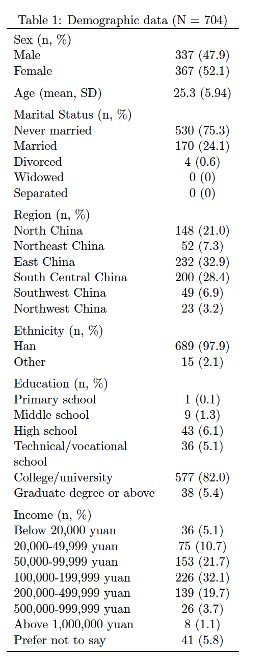
\includegraphics[width=0.2\textwidth]{Picture1.png}
    \caption{Geographic distribution of participants across China}
    \label{fig:latbrain}
\end{wrapfigure}

The final sample comprised 704 participants (337 males, 367 females) with a mean age of 25.3 years (SD = 5.94). The majority of participants (n = 615; 87.4\%) had completed an undergraduate degree, reflecting a highly educated sample. In terms of ethnic composition, the sample was predominantly Han Chinese (n = 689; 97.9\%), while the remaining participants belonged to various ethnic minority groups, including Uygur, Yi, Manchu, Tujia, Zhuang, Bai, and Mongolian. Participants were recruited from diverse geographical regions across China, with over 60\% originating from East China and South Central China, ensuring a broad representation of cultural and regional backgrounds (see Figure~\ref{fig:latbrain}).

\subsection{Validation Framework}
The validation framework employed a comprehensive approach examining multiple psychometric properties through a systematic analysis of validity and reliability measures (see Figure~\ref{fig:TikZmodel}).

\begin{figure}[ht!]
\centering
\begin{tikzpicture}[scale=.5,transform shape,auto,node distance=.9cm,
latent/.style={circle,draw,very thick,inner sep=0pt,minimum size=25mm,align=center},
manifest/.style={rectangle,draw,very thick,inner sep=0pt,minimum width=30mm,minimum height=10mm},
paths/.style={->, ultra thick, >=stealth'}]
\node [manifest] (SI) at (0,0) {criterion validity};
\node [manifest] (VO) [below=of SI] {discriminant validity};
\node [manifest] (CO) [below=of VO] {convergent validity};
\node [manifest] (IN) [below=of CO] {construct validity};
\node [manifest] (WR) [below=of IN] {content validity};
\node [manifest] (BD) [below=of WR] {anxiety};
\node [manifest] (PS) [below=of BD] {depression};
\node [latent] (g) [left=2.5cm of IN] {\emph{g}};
\node [latent] (Gc) [right=4.5cm of CO] {Validity};
\node [latent] (Gv) [right=4.5cm of BD] {Reliability};
\foreach \all in {SI, VO, CO, IN, WR, BD, PS}
{
\draw [paths] (g.east) to node { } (\all.west);
}
\foreach \vc in {SI, VO, CO, IN, WR}
\draw [paths] (Gc.west) to node {} (\vc.east);
\foreach \vs in {BD, PS}
\draw [paths] (Gv.west) to node {} (\vs.east);
\draw [paths, <->] (Gc) edge[bend left] node [left] {} (Gv);
\end{tikzpicture}
\caption{\label{fig:TikZmodel} My TikZ model showing my analysis}
\end{figure}
